\chapter{Method}
\label{chapter:method}
With the theory discussed in the previous chapter it is now possible to build a model for numerical simulations.
Numerical simulations have been at the heart of fluid dynamics for a long time.
This is mainly because of two statements.
On the one hand we can not find an analytical solution to any given flow problem, that has to do with the shape and structure of the Navier-Stokes equations.
In fact there are only a few analytical solutions known. 
They are often referred to as benchmark problems.
One of those is the famous ''Hagen–Poiseuille law'' which is an analytical solution for a flow field in a canal and was first derived by Poiseuille and Haagen in the 18th century~\cite{sutera1993history}.

On the other hand solving differential equations with numerical tools is a story of success.
Long before any computer was build, iterative methods for approximating a solution to a given differential or integral equation have been developed~\cite{}.
Several physics problems are being studied with almost exclusively with numerical tools.
Computational fluid dynamics (CFD) is one of those fields.
Although Moors law has been broken for a few years the computing power is still growing rapidly~\cite{591665}.
Of course instead of ever fast processors, the trend goes in the direction of parallel computing and accelerated computing with accelerator devices such as GPUs.
While GPUs lack the complexity of a CPU they accel at doing simple task over and over again.
As it turns out the lattice Boltzmann method is very well suited to be calculated on the GPU.
The lattice update, which will be explained in the following can be done in parallel for every lattice node, with the exception of boundary nodes.
Therefore in the following the lattice Boltzmann will be introduced, first from a mathematical perspective with it's link to kinetic theory and later from the numerical point of view.

\section{Numerical Methods}\label{sec:numerical_methods}
In this chapter the lattice Boltzmann method will be introduced in great detail.
However one should not forget that lattice Boltzmann method is one among many to simulate the behaviour of a fluid.
Especially when it comes to numerical simulations of the thin film equation, other numerical approaches seem far more established and have been successfully used for more then thirty years.
Since the thin film equation is a fourth order partial differential equation it is usually numerically expensive. 
This is due to the fact that the differential equation is rather stiff and therefor converges very slowly, i.e. needs a lot of iterations.
Still there are finite difference or element schemes that can be used to simulate the thin film equation.
The most used one seems to be the Crank-Nicolson scheme~\cite{crank_nicolson_1947, PhysRevE.63.011208, 10.5555/1403886}.
However all finite difference or element schemes suffer from the concrete choice of discretization.
Since the starting equation is usually defined in continuous space one needs to discretize the system, i.e. introduce a lattice for the computation. 
Assuming full sine wave is shown on a distance of one meter. 
To understand that this curve is a sine it would not be sufficient to have just two points at $x=0$ and at $x=1m$. 
Connecting these two values would  just yield a straight line.
To understand that this curve is a sine at least a few more points are needed.
The same holds true for finite difference, element methods.
One needs a fine enough grid to resolve the important dynamics, but the smaller $h$-the lattice spacing gets the more numerically demanding is the algorithm. 
\begin{figure}
    \centering
    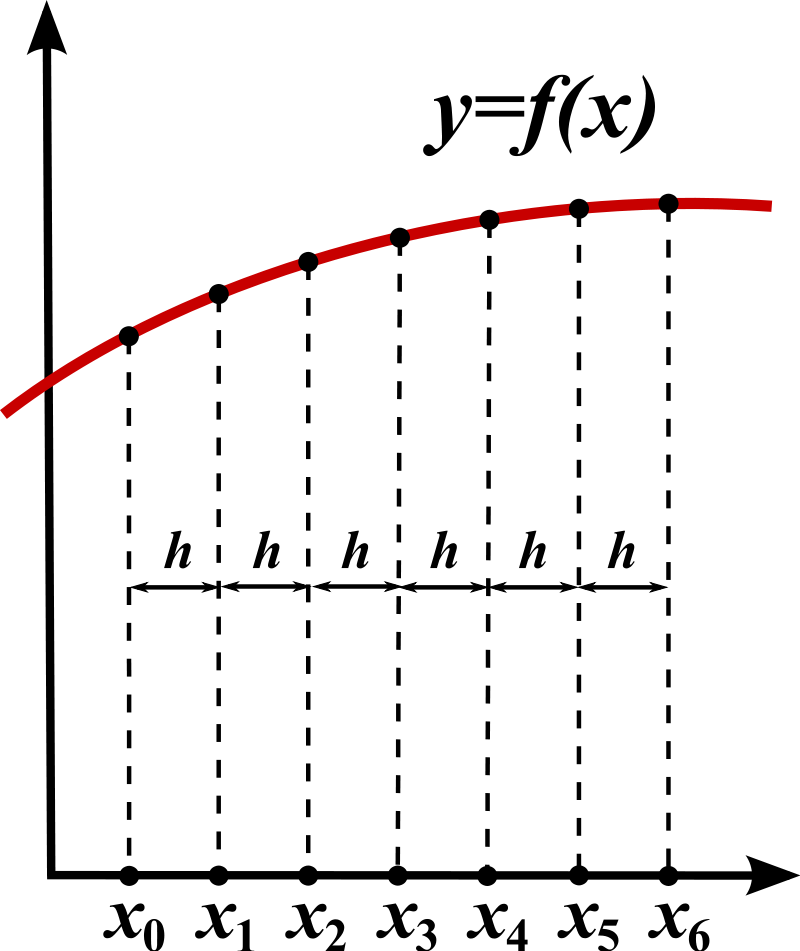
\includegraphics[width=0.5\textwidth]{graphics/800px-Finite_Differences.svg.png}
    \caption{Discretization of a continuous function y (in red) along a disrete space x.
    Each point is the disrete space of x is shifted by the distance h.
    Such the discrete function y of $x\in\{x_0, x_1, x_2, ...\}$ is a straight conection between the dots.}
    \label{fig:finite_difference}
\end{figure}

Of course it is as well possible to perform a transformation and solve in Fourier space, these kind of methods are called Galerkin or discontinous Galerkin methods~\cite{ern2013theory}. 

\section{The Lattice Boltzmann Method}\label{sec:LBM}


The reason why the lattice Boltzmann method is lacking behind when it comes to thin films is that the method in principle always approximated the Navier-Stokes equations.
However the lattice Boltzmann method has strong ties with the CDF community.
Due the simplicity of the method a lot has been worked out over last fourty years.
Since the method got first developed in the 1986 it has gained more and more popularity~\cite{PhysRevLett.56.1505}.

In the first iteration of the lattice Boltzmann method it was yet unclear how many velocities were needed to approximate the Navier-Stokes equations.


\subsection{Lattice Boltzmann for shallow water problems}


\subsection{Thin film flows}
\begin{equation}\label{eq:disjoining_pressure}
    \Pi(h) = \kappa f(h) = = \gamma(1-\cos(\theta))\frac{(n-1)(m-1)}{(n-m)h_{\ast}}\left[\left(\frac{h_{\ast}}{h}\right)^n-\left(\frac{h_{\ast}}{h}\right)^m\right].
\end{equation}